\documentclass[12pt]{report}
\usepackage[utf8]{inputenc}
\usepackage{graphicx}
\usepackage{subcaption}
\usepackage{geometry}
\usepackage{amsmath}
\usepackage{amsthm}
\usepackage{hyperref}
\usepackage{tcolorbox}
\usepackage{minted}
\usepackage{multirow}
\usepackage{multicol}
\geometry{
    left=25mm,
    top=25mm,
    bottom=30mm,
    right=25mm,
}

\newtheorem{theorem}{Theorem}[section]
\newtheorem{claim}[theorem]{Claim}

\begin{document}

\begin{titlepage}
	\centering
	\vspace{1cm}
	{\scshape\Large Assignment 2 \par}
	\vspace{1.5cm}
	{\huge\bfseries COP290 Simulation Report\par}
	\vspace{2cm}
	{\Large\itshape Sayam Sethi 2019CS10399\par}
	{\Large\itshape Mallika Prabhakar 2019CS50440\par}
	\vfill
	supervised by\par
	Prof. Rijurekha Sen
    \vfill
	Department of Computer Science and Engineering\\
	Indian Institute of Technology, Delhi\par
	\vfill

% Bottom of the page
	{\large June 2021\par}
\end{titlepage}

\tableofcontents

\pagenumbering{arabic}

\chapter{Situation}
\section{Story}
Continuing the story from Assignment 2 Task 1, the monopolistic ruling body realised that 1v1 matches are slow and the rate of passing is still high (50\%). The material for vaccine generation was depleting rapidly and they were criticised for killing methods hence they decided to make a different test for analysing worth without involving deaths. They needed lesser percentage of people pass and find the physically and mentally strong people to give vaccines to.

They finally decided on a normal maze game but with some twists. The maze was constructed on a rocky terrain with different sections of maze having different difficulty of traversal. Entire maze will be filled with staining gas (Non toxic gas which gets accumulated in lungs). There will be one time accessible anti-gas chambers which pump out certain quantity of staining gas from their lungs. The person who has the least content of staining gas in lungs is eligible for vaccine and others are barred from getting vaccines. In case of a tie regarding quantity of staining gas, the one who came out earlier will be eligible to obtain the vaccine.

To check mental strength, They give the participants a map marked with terrain difficulty and anti-gas chamber functioning stats along with start and end gate locations as the game starts.

\section{Problem statement}
% random fact: number of Nodes in a n*n maze will be 2 * (n/2)^2 - 1, n > 1 and n is odd
Given a map of the maze denoted with terrain difficulty, anti-gas chamber locations and values and starting and ending points, find and traverse the most efficient route fastest i.e. route which results in least staining gas concentration in lungs. Try to find it in the least time possible as well.

This results in us creating two different algorithms, one with large complexity but the best answer and a faster heuristic approach.

\section{Assumptions}
Following are the general assumptions taken for the development of algorithms.
\begin{itemize}
    \item Players can't jump over walls or take illegal routes
    \item Opponents act fairly and do not affect the game play of others hence are not included in the simulation
    \item The movement speed is considered to be same for all
    \item Each anti gas chamber can be accessed once
\end{itemize}

\section{Mathematical Interpretation of the Problem Statement}

An $n\times n$ sized maze is given with a total of $k$ \textit{special nodes}. Each node $i$ has a weight $w_i$, with the \textit{special nodes} having negative weights and every other node having positive weights. Each  Player starts at the entry gate ($S$). The motive is to find the optimal path to the exit gate ($E$) minimising the value
\begin{equation}
    \sum_{i \in P}{c_i}
\end{equation}
where $P$ is the multi-set of nodes in the path taken from $S$ to $E$ and $c_i=0$ for all occurrences of $i \in K$ (where $K$ is the set of \textit{special nodes}) which is not the first one.

\chapter{Brute Force Approach}
\section{Approach discussion}
The simplest brute force approach is to check all possible situations, i.e., checking over the number of special vertices visited and the order of visiting. Formally stating, the algorithm finds the best path by iterating over all permutations for each element of the power set of the $k$ vertices.\par
The pre-computation would require computing the shortest path for all \textit{special} pairs. This can be easily done using the Floyd-Warshall Algorithm. However, there is a possibility of having cycles with negative path lengths. This can be resolved by first computing the path lengths assuming that the special vertices all have $0$ weights and then adding (the negative) weights of the special vertices $j$ for all ordered ${distance}(i, j)$ pairs. The correctness has been discussed \hyperref[sec:brute-correctness]{below}.\par
The power set can be easily mapped using a bitmask. However, when ordering is introduced, we will need to check all permutations of each mask. This can be efficiently done using a recursive strategy (discussed in the \hyperref[sec:brute-pseudo]{pseudo-code} section).\par
Once we are done with the pre-computation and have decided on a systematic iteration over all possibilities, all that remains is computing the cost of the path for each ordering of each mask which can be easily done using the distance matrix computed earlier.

\section{Pseudo-code}
\label{sec:brute-pseudo}
\subsection{buildGraph}
\begin{tcolorbox}
\begin{minted}{c++}
    // process the graph from the maze
    // initialise the distances (stored as umap<int, umap<int, int>>)
    buildGraph(maze, distances):
      // iterate over all nodes in the maze
      for (node: maze):
        // add an edge for all neighbours to the current node
        for (neighbour: neighbours(node)):
          // if it is a special node, add an edge of weight zero
          // (since negative cycles can exist)
          if (isSpecial(neighbour)):
            addDirectedEdge(node, neighbour, 0)
            distances[node][neighbour] = 0
          else:
            addDirectedEdge(node, neighbour, weight[neighbour])
            distances[node][neighbour] = weight[neighbour]
\end{minted}
\end{tcolorbox}

\subsection{modifiedFloydWarshall}
\begin{tcolorbox}
\begin{minted}{c++}
    // perform regular Floyd-Warshall; then update relevant distances
    modifiedFloydWarshall(distances, specialNodes):
      regularFloydWarshall(distances)
      for (node1: specialNodes):
        distances[S][node1] += weight[node1]
        for (node2: specialNodes):
          if (node1 != node2):
            distances[node1][node2] += weight[node2]
\end{minted}
\end{tcolorbox}

\subsection{enumerateAllPermutations}
\label{pseudo:perms}
\begin{tcolorbox}
\begin{minted}{c++}
    // enumerates all possibities and computes the path length
    enumerateAllPermutations(distances, specialNodes):
      bestDist = INF, ans = []
      for (mask: [0, 1 << k)):
        chosenSpecialNodes = []
        for (i: [0, k)):
          if mask & (1 << i):
            chosenSpecialNodes.add(specialNodes[i])
        sort(chosenSpecialNodes)
        for (permutation: chosenSpecialNodes):
          dist = 0, prevNode = startNode
          for (node: permutation):
            dist += distances[prevNode][node]
            prevNode = node
          dist += distances[prevNode][exitNode]
          if (dist < bestDist):
            bestDist = dist
            ans = permutation
      return (bestDist, ans)
\end{minted}
\end{tcolorbox}

\section {Proof of Correctness}
\label{sec:brute-correctness}

\begin{claim}[property of pairwise distances]
\label{claim:dist-prop}
The \textbf{modified Floyd-Warshall} algorithm computes the correct distances for all pairs of nodes in $\{{startNode}, {endNode}\} \cup K$ (under the assumption that the path is a \textbf{straight path}).
\end{claim}
\noindent(\textbf{Straight path}: A straight path is a path from a node in the set $\{{startNode}, {endNode}\} \cup K$ to another node in the same set which has contribution from every other \textit{special node} equal to $0$ when computing the cost of the path)

\begin{proof}
We know that the weights of the \textit{special nodes} is negative only when we first encounter it.\\
Since we only consider \textit{special paths}, the contribution of every other \textit{special node} to the path length is $0$, which is what we use during the \textit{Floyd-Warshall algorithm}. Additionally, the destination \textit{special node} always contributes to the path length (exactly once) and thus, the shortest path length can be computed as:
\begin{equation}
\begin{aligned}
    &{min}({distance}(u, neighbour)) + {weight}({specialNode})\\
    &= {FloydWarshallDistance}(u, {specialNode}) + {weight}({specialNode})
\end{aligned}
\end{equation}
Hence, the correctness of the \textit{modified Floyd-Warshall} algorithm is proved.
\end{proof}

\begin{claim}[correctness of enumerateAllPermutations]
The \textit{straight paths} computed as defined in \hyperref[claim:dist-prop]{\textbf{claim 2.3.1}} can be used to compute the best path in the function \hyperref[pseudo:perms]{\textbf{enumerateAllPermutations}}.
\end{claim}

\begin{proof}
The function \hyperref[pseudo:perms]{\textit{enumerateAllPermutations}} considers all permutations of every subset of the powerset of the special nodes.\\
Consider the ordered set $B$, which is the set of the the special nodes that are visited in the path with the least cost.\\
It can be shown that the shortest path from $S$ to $E$ which traverses through the nodes in $B$ can be constructed using \textit{straight path} between $S$ and the first element of $B$, \textit{straight paths} between every consecutive element in $B$ and the \textit{straight path} between the last element of $B$ and $E$.\\
Conversely, assume that none of the path between any two consecutive points is not the straight path. Using \hyperref[claim:dist-prop]{\textit{claim 2.3.1}}, the shortest path between the given two nodes is equal to the path length computed by the modified algo since no other special node is visited between the two (otherwise the two nodes would not have been consecutive in the order of visiting).\\
Therefore, the length of the path between these two nodes is larger than the shortest possible path and hence the total path length from $S$ to $E$ would be larger. This is a contradiction to the fact that none of the path is a \textit{straight path}.
Hence, the most optimal path is computed using \hyperref[pseudo:perms]{\textit{enumerateAllPermutations}}.
\end{proof}

\chapter{Faster Solution using Heuristics}

\section{Observations}
The optimal solution has a pre-computation which is very slow and computes a lot of redundant distance values which are never accessed. Only distances from \textit{start node} and \textit{special nodes} are required. Additionally, a lot of the permutations which are processed are clearly suboptimal and their computation should be ignored. For example, going to the farthest \textit{special node} and then coming back to the nearest \textit{special node}, wrt the \textit{start node}.\par
The heuristic that will be discussed aims at optimising primarily on these two aspects. Instead of Floyd-Warshall algorithm, multiple runs of Dijkstra algorithm are done. However, since Dijkstra only works on graphs with non-negative weights, the weights of the special vertices are assumed to be $0$ when performing the algorithm.

<<<<<<< HEAD
\section{Heuristic Algorithm}
The optimised algorithm uses a \textit{greedy} approach by choosing which \textit{special node} to move to next, or directly move to the \textit{exit node}, using the shortest path. The algorithm only considers those \textit{special nodes} which can reduce the path length on visiting, i.e., it considers nodes only if ${distance}({currentNode}, {specialNode}) + {distance}({specialNode}, {exitNode}) < {distance}({currentNode}, {exitNode})$. Out of all these nodes, it chooses the node which is the closest and if there are multiple closest nodes, it chooses the one which offers the least reduction in the cost, if no other vertex was visited. Effectively, the algorithm looks ahead by a single step.
=======
\section{Heuristic Algorithm} % @TODO
The optimised algorithm uses a \textit{greedy} approach by choosing which \textit{special node} to move to next, or directly move to the \textit{exit node}, using the shortest path. The algorithm only considers those \textit{special nodes} which can reduce the path length on visiting, i.e., it considers nodes only if ${distance}({currentNode}, {specialNode}) + {distance}({specialNode}, {exitNode}) < {distance}({currentNode}, {exitNode})$. Out of all these nodes, it chooses the node which is the closest and offers the least reduction in the cost, if no other vertex was visited. Effectively, the algorithm looks ahead by a single step.
>>>>>>> 5a697f1a84c54cee8e3f2f431d39619af53ec564

\section{Pseudo-code}
\subsection{buildGraph}
\begin{tcolorbox}
\begin{minted}{c++}
    // process the graph from the maze
    buildGraph(maze):
      // iterate over all nodes in the maze
      for (node: maze):
        // add an edge for all neighbours to the current node
        for (neighbour: neighbours(node)):
          // if it is a special node, add an edge of weight zero
          // (since Dijkstra doesn't work with negative edges)
          if (isSpecial(neighbour)):
            addDirectedEdge(node, neighbour, 0)
          else:
            addDirectedEdge(node, neighbour, weight[neighbour])
\end{minted}
\end{tcolorbox}

\subsection{computeDistances}
\begin{tcolorbox}
\begin{minted}{c++}
    // compute distances from startNode and all specialNodes
    // to all other specialNodes and exitNode
    computeDistances(graph, startNode, specialNodes):
      // using a hash map to store distances from each source
      // Dijkstra returns the distance vector
      distances[startNode] = Dijkstra(startNode, graph)
      for (node: specialNodes):
        distances[node] = Dijkstra(node, graph)
\end{minted}
\end{tcolorbox}

\subsection{findBestPath}
\begin{tcolorbox}
\begin{minted}{c++}
    findBestPath(graph, distances, specialNodes):
      currentNode = startNode
      pendingSpecialNodes = specialNodes
      while (currentNode != exitNode):
        D = distances[currentNode][exitNode]
        closest = D
        bestCost = D
        bestNode = exitNode
        for (node: pendingSpecialNodes):
          d = distances[currNode][node]
          tot = d + distances[node][exitNode] + weights[node]
          if (tot < D):
<<<<<<< HEAD
            if (d < closest || (d == closest && tot < bestCost)):
=======
            if (d < closest && tot < bestCost):
>>>>>>> 5a697f1a84c54cee8e3f2f431d39619af53ec564
              closest = d
              tot = bestCost
        pendingSpecial.remove(bestNode)
        currNode = bestNode
\end{minted}
\end{tcolorbox}

\chapter{Simulation Display}
\section{Heuristic Slightly sub-Optimal}
\begin{figure}[h]
    \begin{subfigure}{0.5\textwidth}
    \centering
    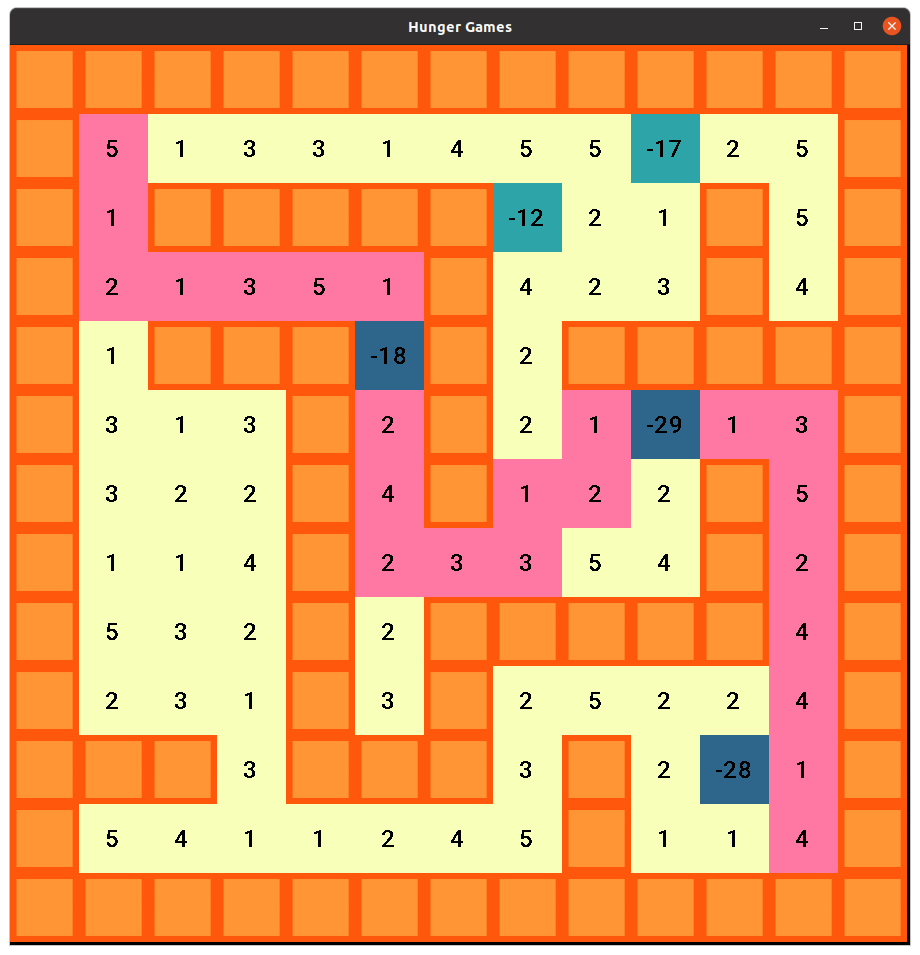
\includegraphics[width=0.9\linewidth]{assets/latex/differentPath/hpath.png}
    \caption{Path chosen by heuristic algorithm (darker vertices are visited); runtime = 0.22s; cost = -19}
    \end{subfigure}
    \begin{subfigure}{0.5\textwidth}
    \centering
    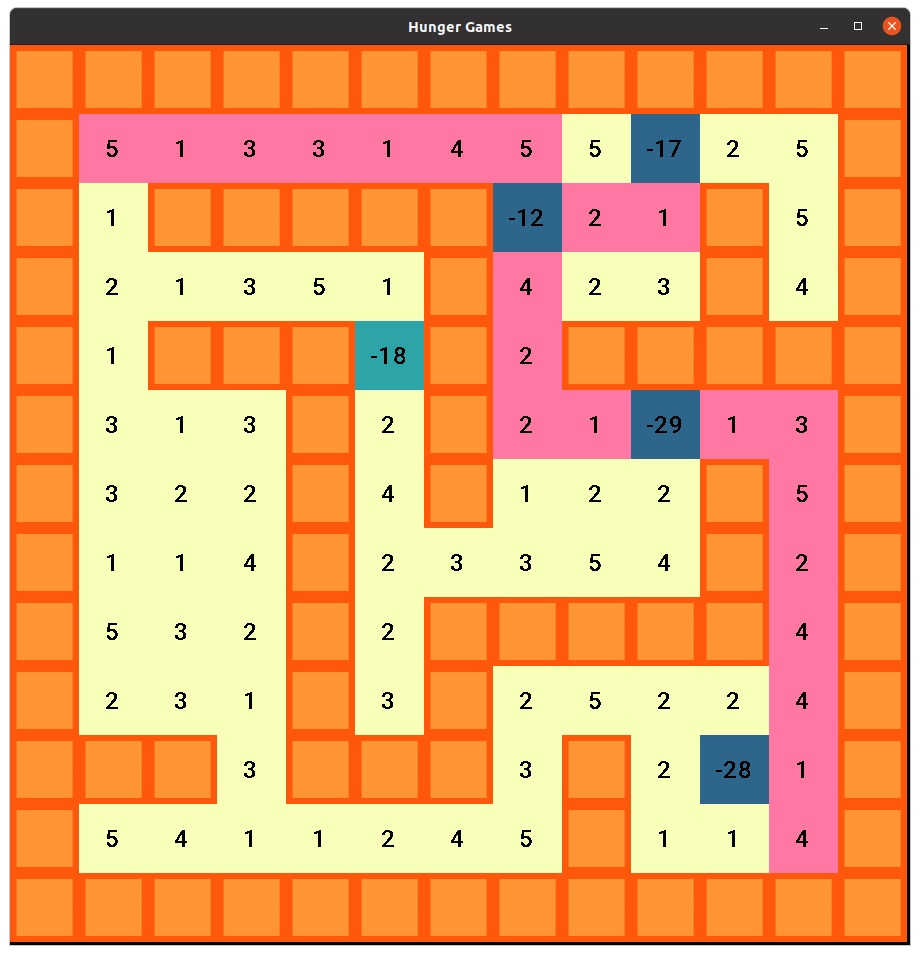
\includegraphics[width=0.9\linewidth]{assets/latex/differentPath/bpath.png}
    \caption{Path chosen by brute force algorithm (darker vertices are visited); runtime = 7.22s; cost = -29}
    \end{subfigure}
\end{figure}
\begin{figure}
    \centering
    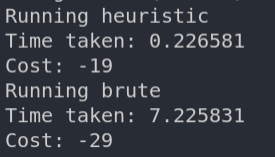
\includegraphics[width=0.4\linewidth]{assets/latex/differentPath/stats.png}
    \caption{Runtime and cost}
\end{figure}

\section{Heuristic Optimal}
\begin{figure}[h]
    \begin{subfigure}{0.5\textwidth}
    \centering
    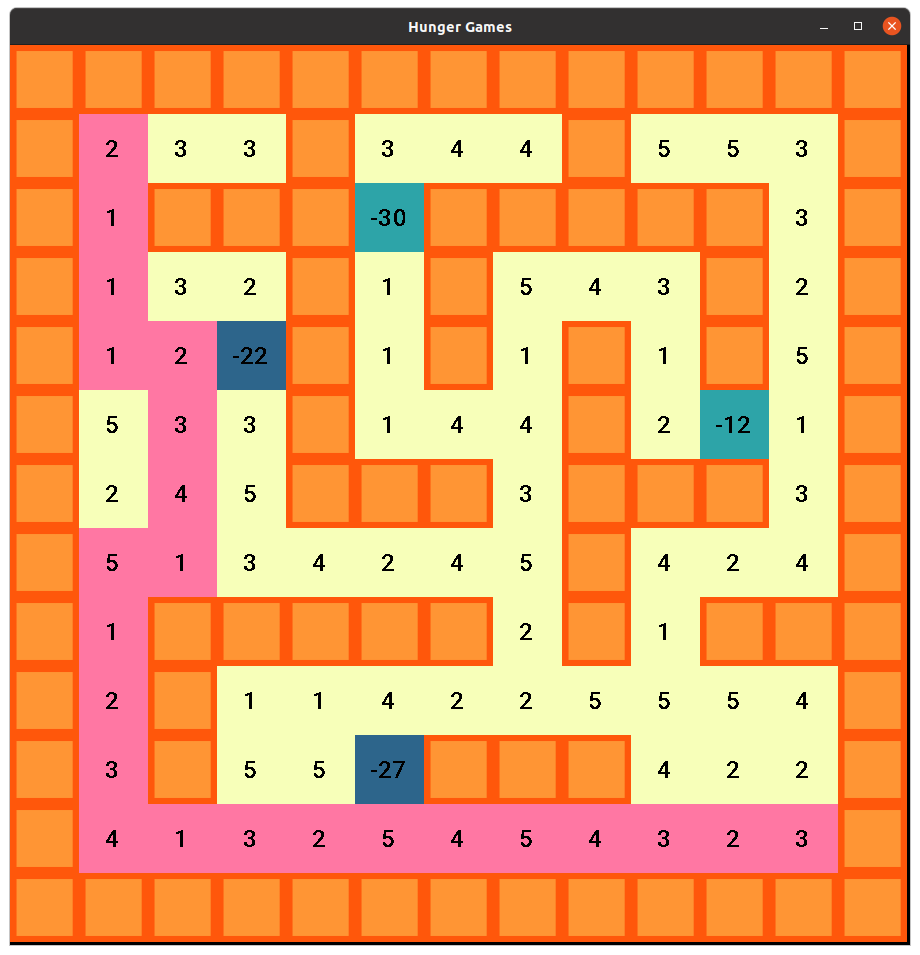
\includegraphics[width=0.9\linewidth]{assets/latex/samePath/hpath.png}
    \caption{Path chosen by heuristic algorithm (darker vertices are visited); runtime = 0.24s; cost = 18}
    \end{subfigure}
    \begin{subfigure}{0.5\textwidth}
    \centering
    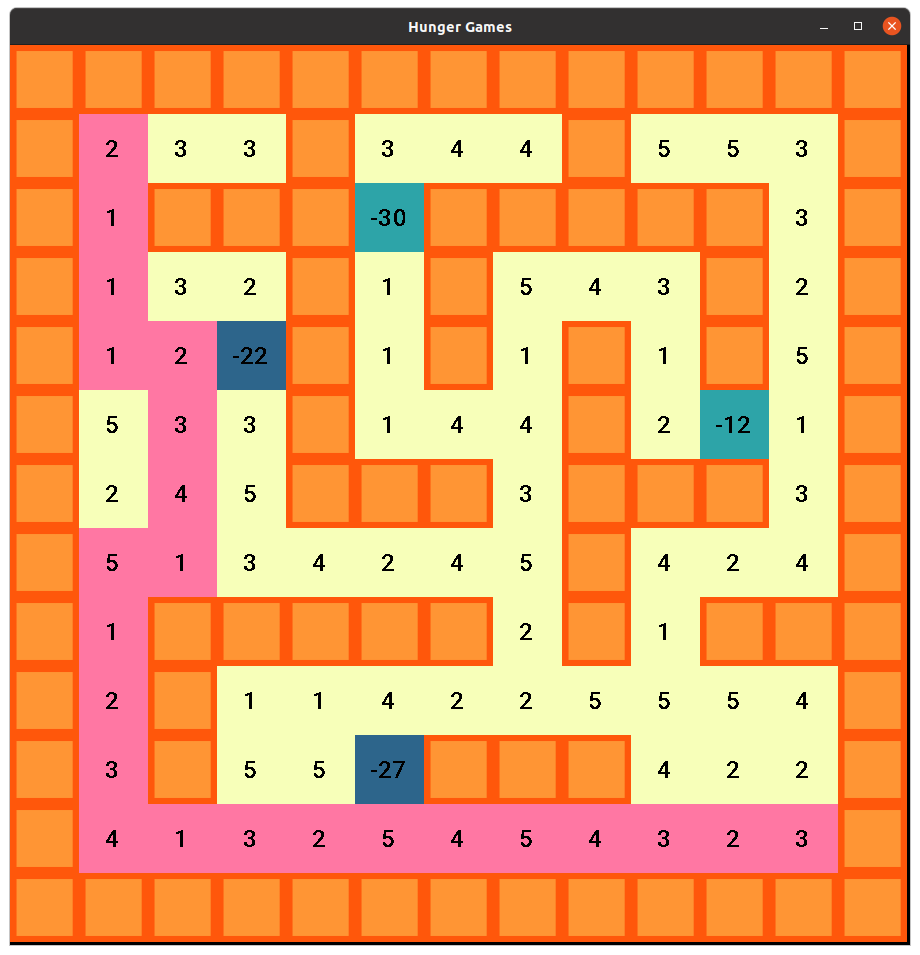
\includegraphics[width=0.9\linewidth]{assets/latex/samePath/bpath.png}
    \caption{Path chosen by brute force algorithm (darker vertices are visited); runtime = 1.53s; cost = 18}
    \end{subfigure}
\end{figure}
\begin{figure}
    \centering
    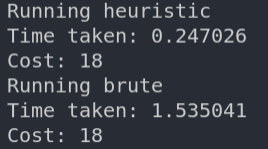
\includegraphics[width=0.33\linewidth]{assets/latex/samePath/stats.png}
    \caption{Runtime and cost}
\end{figure}

\chapter{Analysis}
We are considering the following runtimes by not adding the time taken to generate a maze and set special vertices along with assigning weight to individual vertex.\par
For completeness, following are the time and space complexities of the functions called before calling the brute force and heuristic approaches:

\begin{center}
\begin{tabular}{ |l||c|c| } 
 \hline
 Function name & time complexity &space complexity \\ 
 \hline\hline
 generateSpecialVertices & $O(k)$  & $O(1)$\\
 \hline
 assignWeights & $O(n^2)$& $O(1)$\\ 
 \hline
 backtrack & $O(n^2)$  & $O(1)$\\
 \hline
 generateRandomMaze & $O(n^2)$ & $O(n^2)$ \\ 
 \hline
 removeWalls & $O(n^2)$ & $O(1)$\\ %nothing new 
 \hline
 generateRandomWalls & $O(n^2)$ & $O(n^2)$ \\ %wall array and stack
 \hline
 
\end{tabular}
\end{center}


\section{Runtime analysis for brute force approach}
There are three functions in the brute force approach which are called in succession. Thus the total time complexity is sum of the individual time complexities.
\begin{equation}
\begin{aligned}
    &T({buildGraph}) + T({modifiedFloydWarshall}) + T({enumerateAllPermutations})\\
    &= O(n^4) + O(n^6 + k^2) + O(\sum_{i=0}^{k}{\binom{k}{i}\times(i\times log(i) + i!\times i)})\\
    &= O(n^4) + O(n^6 + k^2) + O(\sum_{i=0}^{k}{\binom{k}{i}\times(i!\times i)})\\
    &= O(n^6 + k! \times k)
\end{aligned}
\end{equation}

\section{Runtime analysis for Heuristic algorithm}
There are three functions in this approach as well which are called in succession. Thus the total time complexity is sum of the individual time complexities.
\begin{equation}
\begin{aligned}
    &T({buildGraph}) + T({computeDistances}) + T({findBestPath})\\
    &= O(n^4) + O(k \times T({Dijkstra})) + O(k^2)\\
    &= O(n^4) + O(k \times (n^2 + n^4 \times log(n^2))) + O(k^2)\\
    &= O(k \times n^4 \times log(n) + k^2)
\end{aligned}
\end{equation}

\section{Comparison of the Two Solutions}
Insert trade-off analysis between error and runtime

\begin{center}
\begin{tabular}{ |c|c||c|c|c|c|c|c| } 
 \hline
 \multirow{2}{*}{n} &
 \multirow{2}{*}{k} & \multicolumn{3}{|c|}{Brute Force} & \multicolumn{3}{|c|}{Heuristic Algorithm}\\
 \cline{3-8}
 & & time taken & cost & chosen cells
 &time taken & cost & chosen cells\\
 \hline\hline
 17 & 8 & $4.187510$ & $-4$ & 5 & $0.009284$ & $-4$ & 5\\
 \hline
 17 & 8 & $5.511454$& $-44$ & 7 & $0.010593$& $-26$& 4\\ 
 \hline
 15 & 3 & $1.364807$ & $33$  & 2& $0.003830$& $33$ & 2\\ 
 \hline
 15 & 3 & $1.443526$& $49$ & 1  & $0.004981$& $52$ & 3\\  
 \hline
 11 & 7 & $0.300426$& $-22$& 6  & $0.004489$& $-22$ &6\\  
 \hline
 11 & 7 & $0.319058$& $-53$  & 6 & $0.004724$& $-45$&4\\
 \hline 
 15 & 4 & $1.389357$& $35$ & 2 & $0.005482$& $35$& 2\\  
 \hline
 15 & 4 & $1.474679$& $-2$ & 3 & $0.004966$& $-2$& 3 \\  
 \hline
 9 & 6 & $0.072333$& $-63$ & 6 & $0.002307$& $-44$& 4 \\  %todo
 \hline
 17 & 2 & $3.298533$& $86$ & 0& $0.003558$& $86$&0 \\  %todo
 \hline
 
\end{tabular}
\end{center}

\section{Observations}

Following observations are made with respect to both the algorithms:
\begin{itemize}
  \item Time take to find the path using brute force algorithm is very large compared to the heuristic approach
  \item Brute force always provides the path of least cost but at a heavy price of time
  \item Heuristic approach does not consider the fact that the path might contains another special vertex hence it provides sub optimal solutions at times
  \item Time complexity of Brute force algorithm is: $O(n^6 + k! \times k)$
  \item Time complexity of Heuristic algorithm is: $O(k \times n^4 \times log(n) + k^2)$
  \item For a large n:k ratio, brute force and heuristic algorithm give similar paths as solution with heuristic algorithm being way faster
  
\end{itemize}



\end{document}
